\chapter{Line Fitting}

\begin{introduction}[Keywords]
    \item 最小二乘法 Least Square Method
    \item 奇异值分解 Singular Value Decomposition (SVD)
    \item 随机抽样一致算法 RANdom SAmple Consensus (RANSAC)
    \item 霍夫变换 Hough Transform
    \item 鲁棒性 Robustness
    \item 离群点 Outliers
    \item 内点 Inliers
\end{introduction}

\section{Least Square Method}

\textbf{最小二乘法} (Least Square Method) :假设有一组数据点 $(x_i, y_i)$,我们希望通过直线 $y = mx + b$ 拟合这些点.

其能量函数(损失函数)为

\begin{equation}
    E=\sum_{i=1}^n(y_i-mx_i-b)^2
\end{equation}

\begin{figure}[htbp]
    \centering
    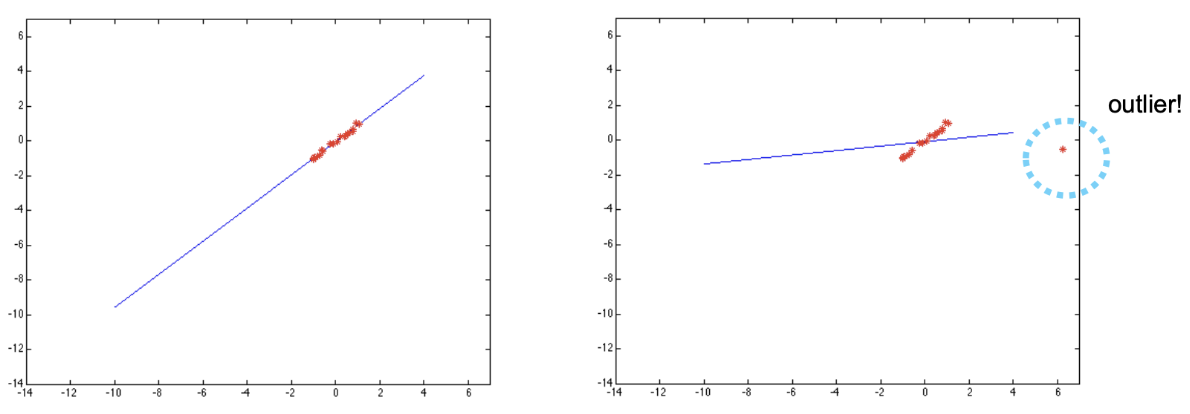
\includegraphics[width=0.8\textwidth]{figures/not_roboust_outliner.png}
    \caption{Least Square Method is not robust to outliers}
\end{figure}

最小二乘法的一个问题是对细微噪声\textbf{鲁棒(robust)}, 但是对于\textbf{离群点(Ouliers)}敏感.

如图,为了照顾一个离群点,整个直线发生了很大的旋转.

\href{http://faculty.bicmr.pku.edu.cn/~wenzw/bigdata/matrix-cook-book.pdf}{Matrix Cookbook} : 记录了很多矩阵求导的公式

\section{Singular Value Decomposition (SVD)}

我们可以将问题重写为矩阵形式.定义数据矩阵 $A$ 和参数向量 $h$:

$$
A = \begin{bmatrix}
x_1 & y_1 & 1 \\
\vdots & \vdots & \vdots \\
x_i & y_i & 1 \\
\vdots & \vdots & \vdots \\
x_n & y_n & 1
\end{bmatrix}, \quad
h = \begin{bmatrix}
a \\
b \\
d
\end{bmatrix}
$$

理想情况下,我们希望解决 $Ah = 0$ 的方程.然而,这通常是一个超定方程组(方程数大于未知数),因此没有精确解.

直接求解 $Ah = 0$ 并不可行,因为存在平凡解 $h = 0$.

所以我们将问题转化为优化问题:

\begin{equation}
    \text{minimize} \: \|Ah\| \: \text{subject to} \: \|h\| = 1
\end{equation}

注意:这里添加约束 $\|h\| = 1$ 而不是强行指定其任一分量为 1,是为了避免排除一些特解(如 x 轴, y 轴, 过原点的直线).

为了解决这个问题,我们将使用奇异值分解(SVD):

$$
A_{n \times 3} = U_{n \times n} D_{n \times 3} V^T_{3 \times 3}
$$

其中:

\begin{itemize}
    \item $U_{n \times n}$ 和 $V_{3 \times 3}$ 是正交矩阵,满足 $V^T V = I_{3 \times 3}$
    \item $V = [c_1, c_2, c_3]$,其中 $c_i$ 是正交向量
    \item $D$ 是对角矩阵,包含奇异值 $\lambda_1, \lambda_2, \lambda_3$,按降序排列 $|\lambda_1| > |\lambda_2| > |\lambda_3|$,也即
    $$
    D_{n \times 3} = \begin{bmatrix}
    \text{diag}\{\lambda_1, \lambda_2, \lambda_3\} \\
    O
    \end{bmatrix}
    $$
\end{itemize}

SVD 是特征值分解在一般矩阵(非方阵)上的扩展.

由于 $V$ 是一个正交阵,所以其列向量构成一组正交基,即 $V_{3 \times 3} = \begin{bmatrix} c_1 & c_2 & c_3 \end{bmatrix}$,其中 $\{c_i\}$ 形成一组正交基,我们可以将 $h$ 表示为:

$$
h = \alpha_1 c_1 + \alpha_2 c_2 + \alpha_3 c_3 = V\begin{bmatrix} \alpha_1 \\ \alpha_2 \\ \alpha_3 \end{bmatrix}
$$

由于 $\|h\| = 1$,我们有 $\alpha_1^2 + \alpha_2^2 + \alpha_3^2 = 1$.

$$
\begin{aligned}
Ah &= U_{n \times n} D_{n \times 3} V^T_{3 \times 3} h_{3 \times 1} \\
&= U_{n \times n} D_{n \times 3} V^T_{3 \times 3} V_{3 \times 3} \begin{bmatrix} \alpha_1 \\ \alpha_2 \\ \alpha_3 \end{bmatrix} \\
&= U_{n \times n} D_{n \times 3} \begin{bmatrix} \alpha_1 \\ \alpha_2 \\ \alpha_3 \end{bmatrix} \\
&= U_{n \times n} \begin{bmatrix} \begin{bmatrix}
\text{diag}\{\lambda_1, \lambda_2, \lambda_3\} \\
O
\end{bmatrix} \begin{bmatrix} \alpha_1 \\ \alpha_2 \\ \alpha_3 \end{bmatrix} \end{bmatrix} \\
&= U_{n \times n} \begin{bmatrix} \text{diag}\{\lambda_1 \alpha_1, \lambda_2 \alpha_2, \lambda_3 \alpha_3\} \\ O \end{bmatrix}
\end{aligned}
$$

再利用 $U$ 是正交矩阵,不影响范数计算的的性质,我们可以得到:

$$
\begin{aligned}
\|Ah\|^2 &= \left\| U_{n \times n} \begin{bmatrix} \text{diag}\{\lambda_1 \alpha_1, \lambda_2 \alpha_2, \lambda_3 \alpha_3\} \\ O \end{bmatrix} \right\|^2 \\
&= \left\| \begin{bmatrix} \text{diag}\{\lambda_1 \alpha_1, \lambda_2 \alpha_2, \lambda_3 \alpha_3\} \\ O \end{bmatrix} \right\|^2 \\
&= (\lambda_1 \alpha_1)^2 + (\lambda_2 \alpha_2)^2 + (\lambda_3 \alpha_3)^2
\end{aligned}
$$

由于 $\alpha_1^2 + \alpha_2^2 + \alpha_3^2 = 1$ 且 $|\lambda_1| > |\lambda_2| > |\lambda_3|$,可以证明:

$$
\|Ah\|^2 \geq \lambda_3^2
$$

等号成立的条件是 $\alpha_1 = \alpha_2 = 0$,$\alpha_3 = 1$,即 $h = c_3$.

SVD 这里的作用在于, 对给定一组数据点, 找到最适配的 k 维子空间, 使得所有数据点到这个子空间的距离最小. 这里我认为王鹤老师讲解地不够本质, 但 SVD 本身非常基础, 可以自行查阅资料.

\section{RANSAC}

RANSAC : RANdom SAmple Consensus, 随机抽样一致算法.

动机: 我们想要一个自动化的算法,可以确定离群点(outliers) 并排除之。

想法: 我们希望找到一个直线, 使得这个直线有最多的内点 (inliner).

\begin{definition}[RANSAC loop]
    假设这个直线需要 2 个点 (或者多一些选为 $n$ 个, 但选择最少的 2 个点可以保证选择的这些点中没有 outliers 的概率最大) 来确定 : 

    \begin{enumerate}
        \item 随机选择 $k$ 组能确定这个直线的点,也就是在所有点里面选出一个 $k\times 2$ 的矩阵
        \item 对每一组点计算出一条直线 (SVD)
        \item 对每一组点的直线计算出所有点到这条直线的距离,如果小于阈值,则认为这个点是这条直线的内点 (inliner)
        \item 找到最大的内点数量的直线,如果大于阈值,则认为这条直线是最优的
        \item 对这个最优的直线,用这个直线所有的内点重新计算一次直线
        \item 重复上述步骤, 直到内点数量不再增加
    \end{enumerate}
    
    注意这里的过程可以很容易地推广到 $n$ 维空间, 只需要选择 $\geq n$ 个点来确定一个 $n-1$ 维的超平面.
\end{definition}
\begin{note}
    实际上从今天来看这个 loop 不需要, 因为我们可以并行地提出所有假设 (Hypothesis), 这里王鹤老师留作作业.
\end{note}

\section{RANSAC calculation}
\begin{problem}
假设我们有所有 inliner 占比为 $w$ 的先验知识,同时希望有不低于 $p$ 的概率能够找到一个最优的直线,那么我们需要多少次迭代呢?
\end{problem}
\begin{proof}
注意到, 
\begin{equation}
\mathbf{\Pr}\text{[一组点全部是inliner]} = w^n
\end{equation}

如果一组点中有一个点是 outliner,那么我们称这组点 fail.

\begin{equation}
\mathbf{\Pr}\text{[k组点全部fail]} = {(1-w^n)}^k
\end{equation}

我们希望 k 组点全部 fail 的概率小于 $1-p$.

\begin{equation}
{(1-w^{n})}^k < 1-p
\Rightarrow
k > \frac{\log(1-p)}{\log(1-w^n)}
\end{equation}
\end{proof}

\section{Hough Transform}

其实就是把一条直线从实际空间的表示转换到参数空间的表示. 但是如果存在垂直的直线, 可能需要考虑使用极坐标来作为参数空间.

\begin{figure}[htbp]
    \centering
    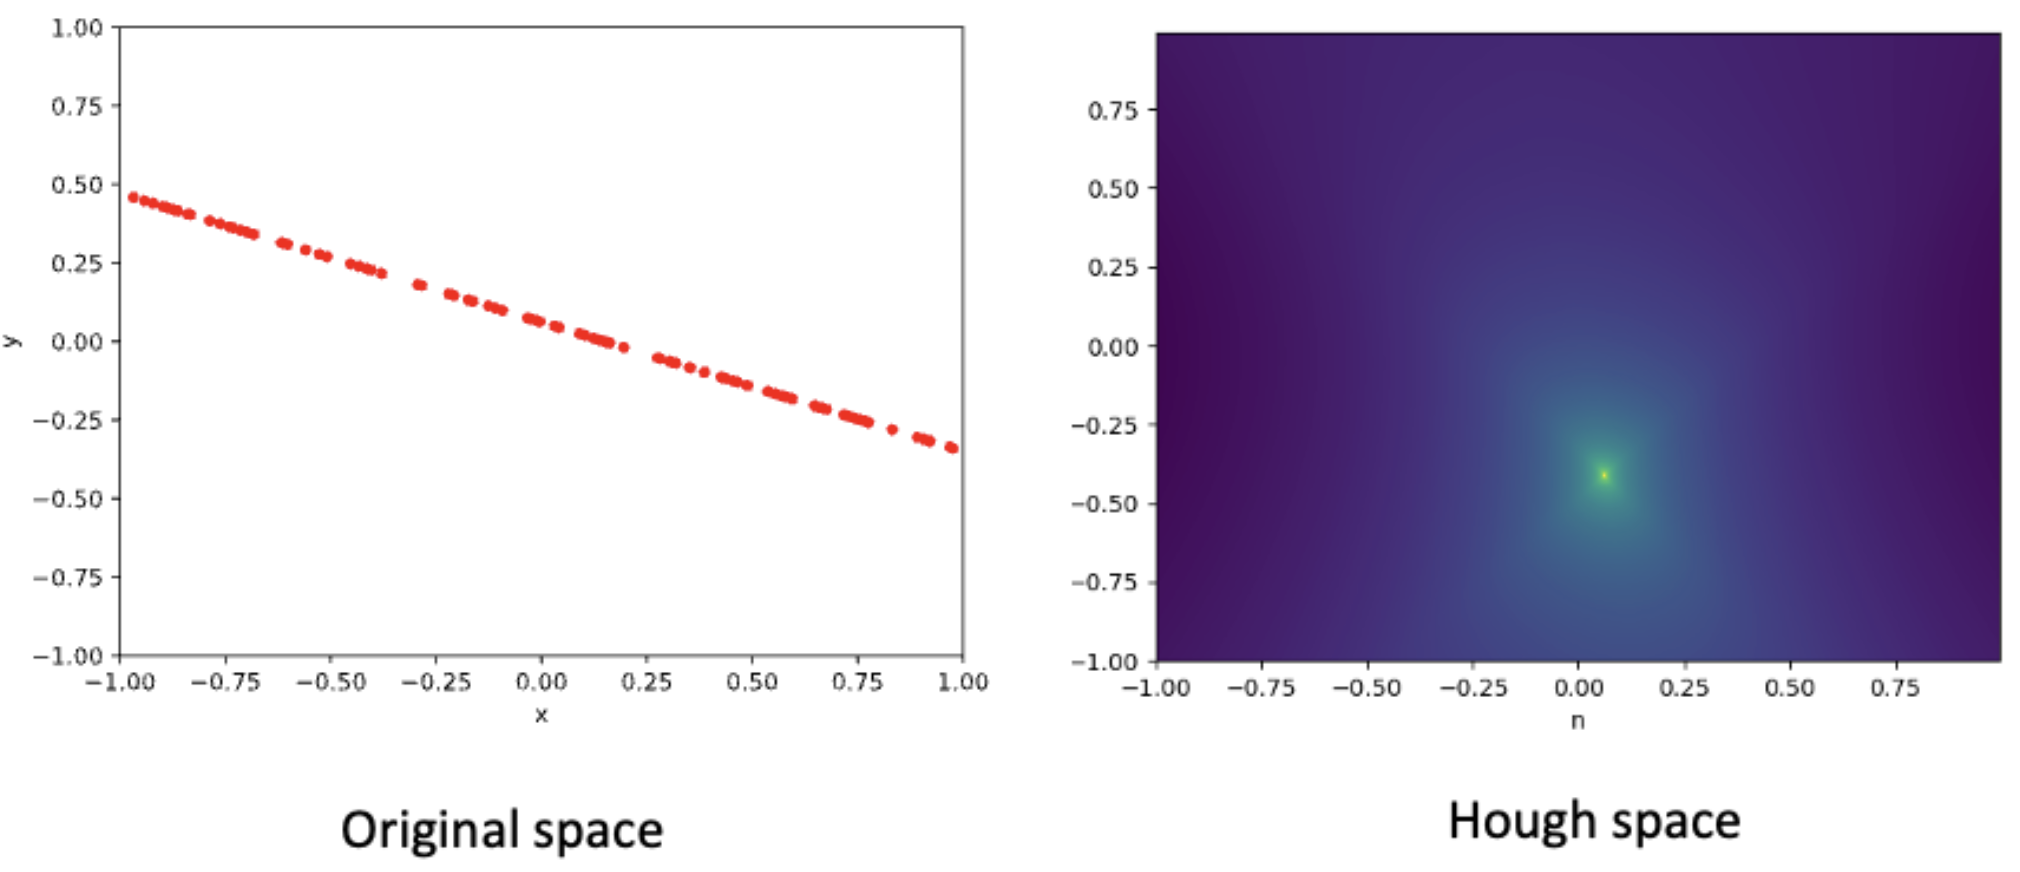
\includegraphics[width=0.8\textwidth]{figures/hough1.png}
    \caption{Hough Transform w/o Noise}
\end{figure}

\begin{figure}[htbp]
    \centering
    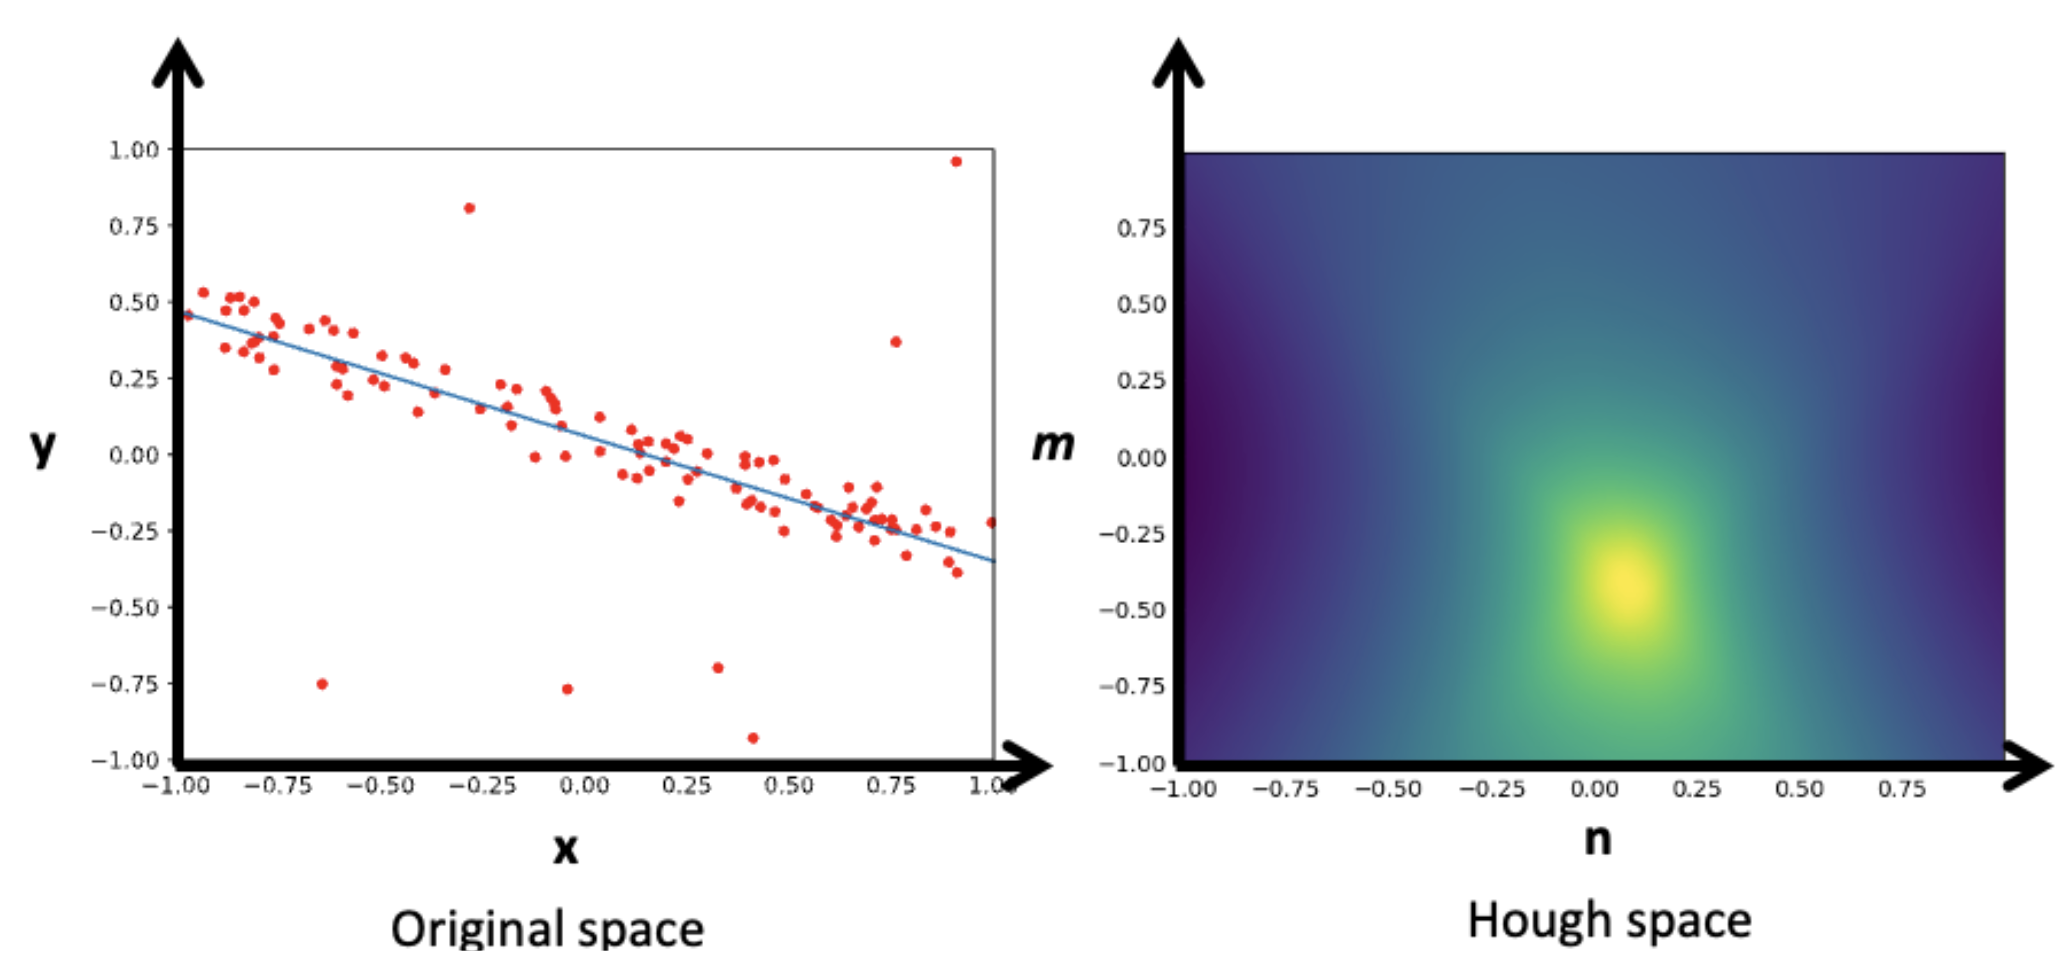
\includegraphics[width=0.8\textwidth]{figures/hough2.png}
    \caption{Hough Transform w/ Noise and Outliers}
\end{figure}